\documentclass[aps,pra,reprint,nofootinbib,superscriptaddress]{revtex4-2}

\usepackage{graphicx}
\usepackage{hyperref}
\usepackage{amsmath, amssymb}
\usepackage{amsthm}
\usepackage{booktabs}

%% Bundle target: D8 (tier 1, journal PRX Quantum | Quantum)
%% Schema: docs/BUNDLE_DIRECTORY_SCHEMA.md
%% Source manifest: papers/D8/source_manifest.md
%% Append log: papers/D8/append_log.json
%% Stage-10 full redraft 2026-08-15. Spine restructured from a nine-item
%% contribution inventory to three questions (existence / length / physical cost),
%% per the Stage-10 prose review. Every headline theorem now appears as a stated
%% theorem rather than a Lean identifier.
%% All headline theorems kernel-pure {propext, Classical.choice, Quot.sound}; 0 project-local axioms.

\newcommand{\lean}[1]{\texttt{#1}}
\newcommand{\su}[1]{\mathrm{SU}(#1)}
\newcommand{\sud}{\mathfrak{su}(d)}
\newcommand{\opn}[1]{\lVert #1 \rVert}

\theoremstyle{plain}
\newtheorem{theorem}{Theorem}
\newtheorem{lemma}[theorem]{Lemma}
\theoremstyle{definition}
\newtheorem{definition}[theorem]{Definition}
\newtheorem{hypothesis}[theorem]{Hypothesis}

%% ═══════════════════════════════════════════════════════════════════
%% \figuredeferred{id}{reason} — the declared-deferral form
%% ═══════════════════════════════════════════════════════════════════
%%
%% WAVE_EXECUTION_PIPELINE.md §Stage 9: "A figure that is planned but not yet
%% drawn is declared with \figuredeferred{id}{reason}, never omitted silently."
%% The law mandated this form and, measured 2026-08-09, it had ZERO uses across
%% all 21 bundle drafts — nine of which carried no figures at all. Nine bundles
%% with no plan is a charter defect; nine bundles with a *stated* plan and a
%% stated blocker is an honest manuscript in progress, and a referee can tell
%% the two apart only if the plan is on the page.
%%
%% The deferral is DELIBERATELY VISIBLE in the compiled PDF. A silent macro
%% would satisfy `bundle_figure_adequacy` while showing a reader nothing, which
%% is the vacuous-Stage-9 failure ("ALL figures PASS" over an empty set) rebuilt
%% one layer up.
%%
%% ⚠️ The reason must name what BLOCKS the figure, not that it is absent.
%% "not yet drawn" is boilerplate and defeats the purpose; "awaiting the L=8
%% m→0 production run" is a blocker a reader can check and a later pass can
%% discharge.
%%
%% Definition lives here, beside docs/counts.tex, because 21 drafts consume it
%% and a per-draft copy is 21 places for the rendering to drift.

%% Rendered as a non-floating box on purpose. A `figure` float would be subject
%% to revtex's two-column placement rules across eleven drafts for no gain, and
%% a deferral does not need a figure number: it is a promise, not a result.

\providecommand{\figuredeferred}[2]{%
  \par\medskip\noindent
  \fbox{\parbox{0.92\columnwidth}{%
    \small\textbf{Figure deferred: \texttt{#1}.}
    Planned for this section; not yet produced. \emph{Blocked on:} #2.%
  }}%
  \par\medskip
}


\begin{document}

\title{Kernel-Verified Universal Quantum Gate Compilation:\\
Alphabet-Agnostic Solovay--Kitaev across Dimensions}

\author{John Roehm}

\begin{abstract}
We prove, in the Lean~4 proof assistant and checked to the kernel, a
quantitative Solovay--Kitaev theorem at arbitrary dimension: for a generating
set of $\su d$ that is dense and has compatible word length, every target
$U \in \su d$ and every precision $\varepsilon$ below a fixed threshold admit a
word approximating $U$ within $\varepsilon$ whose length is at most
$c\,(\log 1/\varepsilon)^{\gamma}$ with $\gamma = \log 5/\log(3/2)$, both bounds
holding of the same compiled word. To our knowledge this is the first
kernel-verified quantitative Solovay--Kitaev theorem at general dimension in
any proof assistant; the enabling step is a Banach-algebra matrix logarithm
with an explicit convergence radius, which removes a circular dependency that
blocks the naive lift. Because the two hypotheses are the only alphabet-specific
input, a gate set enters the verified theory by supplying a density witness, and
we discharge four such witnesses, at $\su 2$, $\su 4$ and $\su 8$. At $\su 8$ we
settle the role of the doubly controlled-$Z$ gate: it is sufficient for density
with no $T$ gate present, it is necessary, since the Clifford group alone has
finite image under the channel representation, and it is priced, by a
machine-checked lower bound on the number of Toffoli gates in any exact
Clifford$+$CCZ circuit for a target. Beyond existence we verify a named
correct-by-construction Clifford$+T$ compiler; two further length mechanisms
attaining the optimal $O(\log 1/\varepsilon)$, one conditional on a stated
number-theoretic hypothesis and one unconditional with ancillas; and an
end-to-end certificate converting compiler accuracy $\varepsilon$ into
worst-case channel error at most $\sqrt 2\,\varepsilon$. All results use the
standard Lean axiom set with no project-local axioms and no compiled-evaluation
escapes. Runtime implementation, hardware tuning and constant-factor length
optimization are outside this scope.
\end{abstract}

\maketitle

\section{Introduction}
\label{sec:intro}

A compiler for a quantum processor answers three questions about every target
unitary it is handed. Does a circuit over the machine's gate set approximate
this target at all? How long is that circuit? And what does running it cost, in
the error budget the hardware actually charges against? The Solovay--Kitaev
theorem answers the first affirmatively for any sufficiently rich gate set and
gives a poly-logarithmic answer to the second, and both answers are, in the
literature, proved one gate set at a time.

This paper reports a machine-checked development, in the Lean~4 proof
assistant, that answers all three, and that answers the first in a form which
is reusable rather than per-alphabet. Its organizing observation is that of the
ingredients in a Solovay--Kitaev proof, only one is alphabet-specific. The
density argument that a discrete gate set does not close up into a finite group
depends on the gate set. The $\varepsilon_0$-net, the balanced group-commutator
recursion, the Baker--Campbell--Hausdorff estimate controlling it, and the
Cartan step from a one-parameter subgroup to the whole group do not. Separating
them yields a substrate over an abstract generating set, into which an alphabet
enters by supplying a density witness and nothing else
(Sec.~\ref{sec:substrate}), and which lifts to the special unitary group
$\su d$ of arbitrary dimension once an obstruction involving convergence radii
is removed (Sec.~\ref{sec:sud}). To our knowledge, the resulting statement is
the first kernel-verified quantitative Solovay--Kitaev theorem at general
dimension in any proof assistant.

Sec.~\ref{sec:alphabets} is the evidence for the reusability claim rather than
a survey: four alphabets, whose density witnesses range over an
algebraic-integer obstruction, a Chebyshev factorization, a triple-angle
identity and an entangling-gate criterion, all pass through the interface
without modifying it. Sec.~\ref{sec:su8} treats the three-qubit case at length,
because there the question of which gate carries the universality has a
complete answer: the doubly controlled-$Z$ gate is necessary, is sufficient
without any $T$ gate, and has a machine-checked cost, all three established
through the channel representation.

The second question, circuit length, is Sec.~\ref{sec:length}. Three verified
mechanisms reach it, and none dominates: the commutator recursion is
unconditional at exponent $\approx 3.97$; the Ross--Selinger grid
route~\cite{RossSelinger2016} reaches the optimal exponent $1$ but rests on a
number-theoretic existence that is open, which we isolate as a single stated
hypothesis rather than an atmosphere of caveats; and the
Kliuchnikov--Maslov--Mosca ancilla route~\cite{KMM2013ancilla} reaches exponent
$1$ unconditionally, at the price of two ancillas and a weaker form of
contract. Between the first and second questions sits a third thing a compiler
user wants and an existence theorem does not give: Sec.~\ref{sec:compiler}
verifies a named compilation \emph{function}, whose error and length bounds are
theorems about the algorithm rather than certificates checked per output.

The third question is Sec.~\ref{sec:diamond}, which converts a bound between
matrices into a bound between physical channels and composes it with the
verified compiler, so that a synthesis accuracy $\varepsilon$ yields a
worst-case channel error at most $\sqrt 2\,\varepsilon$ with no unverified step
in between.

Prior formal verification in quantum computation has largely targeted
\emph{exact} circuit semantics. VOQC and SQIR in Coq~\cite{Hietala2020VOQC}
verify that circuit optimizations preserve semantics, and the wider landscape
of verified quantum programming, including Why3/Qbricks and Isabelle
developments, is surveyed in Ref.~\cite{Lewis2021VerifQC}. Those establish that
a circuit computes what it should. The subject here is different and
complementary: quantitative \emph{approximation}, meaning the density of a
discrete alphabet, the trade-off between error and length, and resource lower
bounds. Verifying that a given circuit is correctly optimized and verifying
that a target can be approached to arbitrary precision within a length budget
are different questions, and the second is the one a compiler's existence
guarantee rests on.

Sec.~\ref{sec:trust} states what the kernel checked and, more usefully, the
places where a theorem's name reads stronger than the theorem. All results are
verified with the standard Lean axiom set and no project-local axioms, and the
corpus contains no compiled-evaluation escape hatch.
Table~\ref{tab:results} is the map.

\begin{table}
\caption{The results, and where each is proved. Conditional statements carry
their hypotheses in the theorem statement; unconditional ones have none.}
\label{tab:results}
\begin{ruledtabular}
\begin{tabular}{llc}
Result & Statement & Conditional \\
\colrule
SK over an abstract alphabet & Thm~\ref{thm:substrate} & yes \\
Logarithm with named radius & Thm~\ref{thm:mercator} & no \\
SK at arbitrary $\su d$ & Thm~\ref{thm:sud} & yes \\
Clifford$+T$ density & Thm~\ref{thm:accpt} & no \\
Clifford$+T$ compilation & Thm~\ref{thm:cliffordt} & no \\
$T$-free density at $\su 8$ & Thm~\ref{thm:literal} & no \\
Clifford-only is not dense & Thm~\ref{thm:notdense} & no \\
Toffoli-count lower bound & Thm~\ref{thm:toffoli} & no \\
Compiler correctness & Thm~\ref{thm:compile} & no \\
Grid-route length, exponent $1$ & Thm~\ref{thm:rslength} & yes \\
Grid route from the hypothesis & Thm~\ref{thm:rssynth} & yes \\
Ancilla route, exponent $1$ & Thm~\ref{thm:kmm} & no \\
Operator norm to diamond & Thm~\ref{thm:akn} & no \\
End-to-end channel certificate & Thm~\ref{thm:capstone} & no \\
\end{tabular}
\end{ruledtabular}
\end{table}

\section{Compilation as an instantiable theory}
\label{sec:substrate}

A quantum processor exposes a fixed, finite set of physical gates and must
approximate an essentially continuous family of target unitaries. The
Solovay--Kitaev theorem guarantees that any sufficiently rich gate set can do
so to precision $\varepsilon$ with a circuit whose length grows only
poly-logarithmically in $1/\varepsilon$~\cite{KitaevShenVyalyi2002,DawsonNielsen2006,AharonovArad2011}.
Its proof combines three ingredients that are usually presented together and
proved together for one gate set at a time: a Lie-theoretic argument that the
generated group is dense, a geometric recursion on the group manifold near the
identity, and a number-theoretic obstruction establishing that the discrete
alphabet does not close up into a finite group.

Only the third of these is alphabet-specific. That observation is the
organizing principle of this work, and the substrate below is what it buys:
the first two ingredients are proved once, quantified over an abstract gate
set, and a new alphabet inherits a quantitative compiler by supplying a single
density witness.

\subsection{The interface}
\label{sec:substrate-interface}

The abstraction an alphabet must satisfy is deliberately thin. It is a group
of formal words together with a representation into the target group, and a
finite generating set for that group of words.

\begin{definition}[Generating set]
\label{def:gs}
A \emph{generating set} for $\su d$ is a structure $\mathrm{gs}$ consisting of:
a type $W$ carrying a group structure (the formal words); a group homomorphism
$\rho \colon W \to \su d$ (the interpretation of a word as a unitary); a finite
subset $\mathrm{gens} \subseteq W$; a proof that $\mathrm{gens}$ is non-empty;
and a proof that $\mathrm{gens}$ generates $W$, that is
$\langle \mathrm{gens}\rangle = W$.
\end{definition}

Nothing in Definition~\ref{def:gs} refers to matrices of a particular shape, to
a braid group, to a Clifford hierarchy, or to a dimension larger than the one
in the ambient $\su d$. Two predicates over such a structure carry the whole
argument.

\begin{definition}[Density witness]
\label{def:dense}
$\mathrm{gs}$ is \emph{dense} when for every $U \in \su d$ and every
$\varepsilon > 0$ there is a word $w \in W$ with
$\opn{\rho(w) - U} < \varepsilon$.
\end{definition}

\begin{definition}[Word-length compatibility]
\label{def:wordlen}
A length function $\ell \colon W \to \mathbb{N}$ is \emph{free-group-like} when
it satisfies the sub-additivity and inversion bounds that the balanced
commutator construction consumes, so that the length of a composite word is
controlled by the lengths of its parts.
\end{definition}

Throughout, $\opn{\cdot}$ is the $\ell^\infty$ operator norm on matrices (the
maximum absolute row sum), which is the norm the formalization carries. This
matters in Sec.~\ref{sec:diamond}, where converting to a channel-level
statement requires passing to the $\ell^2$ operator norm and pays an explicit
dimensional constant to do so.

\subsection{What the substrate proves}

The substrate's content is that Definitions~\ref{def:dense}
and~\ref{def:wordlen} are jointly sufficient. Everything else in the
Solovay--Kitaev argument is discharged once and reused.

\begin{theorem}[Quantitative Solovay--Kitaev over an abstract alphabet]
\label{thm:substrate}
Let $\mathrm{gs}$ be a generating set for $\su d$ whose word type is a free
group, let $\mathrm{gs}$ be dense in the sense of Definition~\ref{def:dense},
and let its free-group word length be compatible in the sense of
Definition~\ref{def:wordlen}. Then there exist $\varepsilon_0 > 0$, a constant
$c > 0$, and a function
$\mathrm{compile} \colon \su d \times \mathbb{R} \to W$
such that for every $U \in \su d$ and every $\varepsilon \in (0, \varepsilon_0]$,
\[
  \opn{\rho\big(\mathrm{compile}(U,\varepsilon)\big) - U} \;\le\; \varepsilon
  \qquad\text{and}\qquad
  \lvert \mathrm{compile}(U,\varepsilon)\rvert \;\le\;
    c\,\big(\log (1/\varepsilon)\big)^{\gamma},
\]
where $\lvert\cdot\rvert$ is the reduced free-group word length and
$\gamma = \log 5/\log(3/2)$.
\end{theorem}

Two features of Theorem~\ref{thm:substrate} are worth isolating, because they
are what a compilation pipeline actually needs and what existence-only
statements of the Solovay--Kitaev theorem do not supply. First, the two bounds
hold \emph{at the same compile level}: the same $\mathrm{compile}(U,\varepsilon)$
witnesses both, rather than one word being short and a different word being
accurate. Second, the length bound is on the reduced word that the construction
emits, not on an auxiliary counter. Sec.~\ref{sec:compiler} returns to this
point, because at $\su 2$ the substrate's own length conjunct is stated for the
recursion-level length function and the bound on the emitted word is a separate,
later theorem.

\subsection{The mechanism, and its constants}
\label{sec:substrate-mechanism}

Four ingredients sit behind Theorem~\ref{thm:substrate}, and none mentions the
alphabet.

The \emph{$\varepsilon_0$-net} supplies a finite family of words approximating
every target to a fixed base precision $\varepsilon_0$. Density
(Definition~\ref{def:dense}) plus compactness of $\su d$ gives one.

The \emph{balanced group-commutator recursion} of Dawson and
Nielsen~\cite{DawsonNielsen2006} is the engine. Given a word $W_n$ with
$\opn{\rho(W_n) - U} \le \varepsilon_n$, write the residual
$\Delta = U\rho(W_n)^{-1}$, which is within $\varepsilon_n$ of the identity.
Write $\Delta = \exp(H)$ with $H$ traceless anti-Hermitian and
$\opn{H} = O(\varepsilon_n)$, split $H$ as a Lie bracket $[A,B]$ with
$\opn{A},\opn{B} = O(\sqrt{\varepsilon_n})$, approximate $\exp(A)$ and
$\exp(B)$ recursively, and take the group commutator of the results. The gain
is the discrepancy between the group commutator and the exponential of the Lie
bracket, which is third order in the operand norms and hence
$O(\varepsilon_n^{3/2})$ in the residual. The cost is that $W_{n+1}$ is built
from five level-$n$ words.

The \emph{Baker--Campbell--Hausdorff estimate} is what makes the previous
sentence a theorem. It bounds
$\opn{\exp(A)\exp(B)\exp(-A)\exp(-B) - \exp([A,B])}$ by a cubic in
$\max(\opn A, \opn B)$, with an explicit constant, at order two.

The \emph{Cartan step} converts an accumulation point at the identity into
density: an infinite-order element in a compact group generates a subgroup
whose closure contains a one-parameter subgroup, whose generator spans a line
in the Lie algebra, and conjugation spreads that line to the whole algebra.

The two recurrences these produce are
\[
  \varepsilon_{n+1} = K^{2}\varepsilon_n^{3/2},
  \qquad
  L(n+1) = 5\,L(n) + \beta ,
\]
with $K = 1024$ the composition constant of the estimate above and $\beta$ the
per-level assembly overhead. They solve in closed form to
$L(n) = \lambda\,5^n + \beta(5^n - 1)/4$, and the base threshold is
$\varepsilon_0 = 1/(8K^2)$, chosen so that $K^2 \cdot 2\varepsilon_0 = 1/4 < 1$,
which is the condition under which the error recurrence contracts. In the
formalization $\lambda = \beta = 100$ and $c = 1000$; these are rigorous upper
bounds rather than tight ones, and Sec.~\ref{sec:length} is where tightness is
pursued by other means.

The $\varepsilon_0$-net deserves an explicit caveat. In the generic substrate it
is obtained existentially from the density witness rather than by enumeration,
so Theorem~\ref{thm:substrate} asserts that a compilation \emph{exists} with the
stated bounds and does not exhibit a procedure that emits it. That gap is closed
for one alphabet, and only one, in Sec.~\ref{sec:compiler}.

\subsection{The alphabet-specific residue, worked once}
\label{sec:substrate-cliffordt}

What an alphabet must supply is a density witness, and in practice the density
witness reduces to showing that some word has infinite order. We work the
canonical fault-tolerant case, Clifford$+T$, in full, because it is the pattern
every later alphabet reuses.

Let $H_{\mathrm{SU}}$ and $T_{\mathrm{SU}}$ be the determinant-one
representatives of the Hadamard and $T$ gates. The trace of the product is
$\sqrt 2\,\sin(\pi/8)$. Were the product of finite order, its eigenvalues would
be roots of unity and its trace an algebraic integer, being a sum of two roots
of unity. It is not: $\sqrt 2\,\sin(\pi/8)$ has minimal polynomial with
non-monic integral scaling, so it fails to be an algebraic integer, and the
element therefore has infinite order. Since $\su 2$ is compact, the closure of
the group generated by an infinite-order element contains a limit point at the
identity.

\begin{theorem}[Accumulation at the identity for $\langle H, T\rangle$]
\label{thm:accpt}
The identity is an accumulation point of the subgroup of $\su 2$ generated by
the Clifford$+T$ alphabet.
\end{theorem}

Theorem~\ref{thm:accpt} is the sole alphabet-specific input, and it is
unconditional. Feeding it through the Cartan argument yields density, and
feeding density through Theorem~\ref{thm:substrate} yields the compiler
statement for Clifford$+T$ with no residual hypothesis.

\begin{theorem}[Clifford$+T$ compilation]
\label{thm:cliffordt}
For every $U \in \su 2$ and every $\varepsilon \in (0,\varepsilon_0]$, the
Clifford$+T$ compilation of $U$ at precision $\varepsilon$ satisfies
$\opn{\rho(\mathrm{compile}(U,\varepsilon)) - U} \le \varepsilon$, and the
level-$n$ length bound $L(n) \le c\,(\log 1/\varepsilon)^{\gamma}$ holds at
$n = n(\varepsilon)$, the recursion depth the compiler runs to.
\end{theorem}

The route from an algebraic-integer obstruction to a quantitative compiler is
the reusable one. The next two sections extend it in the two directions a
compilation pipeline cares about: to higher dimension, and to other alphabets.

\section{The lift to arbitrary dimension}
\label{sec:sud}

Single-qubit compilation is $\su 2$. A pipeline targeting $n$ qubits needs
$\su{2^n}$, and there is no reason for the theory to be dimension-specific.
Lifting Theorem~\ref{thm:substrate} from $\su 2$ to $\su d$ is mostly routine:
the net, the recursion and the Cartan step all generalize. One step does not,
and it is worth exhibiting the obstruction because removing it is the technical
core of this section.

\subsection{Why the naive lift is circular}

The balanced commutator construction, at each level, takes a near-identity
unitary $\Delta$ and writes it as $\exp(H)$ for a traceless anti-Hermitian $H$
of controlled norm, then approximates $H$ by a Lie bracket and reassembles. At
$\su 2$ one may write the logarithm down by hand. At general $d$ the natural
tool is the inverse function theorem applied to the matrix exponential at the
identity, which yields a local homeomorphism on \emph{some} neighbourhood.

The neighbourhood is the problem. The inverse function theorem supplies a radius
$r$ existentially, and the recursion needs to know that the level-$(n+1)$
residual falls inside it. But the level-$(n+1)$ residual is bounded in terms of
the level-$n$ construction, which used the logarithm, which required a radius.
Discharging the level-$(n+1)$ regime hypothesis therefore requires a bound
established using the very radius whose applicability is in question, and the
dependency does not terminate. An existential radius cannot be threaded through
an induction whose inductive step consumes it.

\subsection{A logarithm with a named radius}

We break the circle by not using the inverse function theorem. On a Banach
algebra the Mercator series converges on an explicit ball, and matrices under
the $\ell^\infty$ operator norm form one.

\begin{theorem}[Matrix logarithm with an explicit radius]
\label{thm:mercator}
Define
\[
  \log_{\mathrm{M}} X \;=\; \sum_{n \ge 0} \frac{(-1)^n}{n+1}\,X^{n+1}.
\]
For every $d$ and every $X \in \mathbb{C}^{d\times d}$ with $\opn{X} < 1$, the
series converges and
$\exp\big(\log_{\mathrm{M}} X\big) = \mathbf 1 + X$.
\end{theorem}

The radius is $1$, stated in the theorem, uniform in $d$, and independent of
anything the recursion computes. With Theorem~\ref{thm:mercator} in hand each
regime conjunct (that the logarithm is anti-Hermitian, that it is traceless,
and that the exponential round trip holds) is discharged on a named ball, and
the induction closes. Mathlib carries the scalar and Banach-algebra exponential
but no logarithm with a named convergence radius, so
Theorem~\ref{thm:mercator} fills a gap in the underlying library rather than
only in this development.

\subsection{The general-dimension theorem}

\begin{theorem}[Quantitative Solovay--Kitaev at arbitrary dimension]
\label{thm:sud}
Let $d \ge 2$ and let $\mathrm{gs}$ be a generating set for $\su d$ over a free
word group. If $\mathrm{gs}$ is dense and its word length is compatible, then
the conclusion of Theorem~\ref{thm:substrate} holds at dimension $d$: there
exist $\varepsilon_0, c > 0$ and a compilation function meeting the error bound
$\varepsilon$ and the word-length bound
$c\,(\log 1/\varepsilon)^{\gamma}$ simultaneously, for every target in $\su d$
and every precision in $(0,\varepsilon_0]$.
\end{theorem}

To our knowledge Theorem~\ref{thm:sud} is the first machine-checked
quantitative Solovay--Kitaev statement at general dimension in any proof
assistant. It is stated conditionally on the two interface predicates, which is
the point: the conditions are exactly what an alphabet supplies, and
Sec.~\ref{sec:alphabets} discharges them at $d = 4$ and $d = 8$, where the
resulting compilation theorems are unconditional.

\subsection{The exponent}
\label{sec:sud-exponent}

The recursion contracts error as $\varepsilon \mapsto O(\varepsilon^{3/2})$
while expanding word length fivefold per level. Solving the pair gives a
recursion depth $n(\varepsilon) = \log_{3/2}\log(1/\varepsilon)$ and a length
$5^{n(\varepsilon)} = (\log 1/\varepsilon)^{\gamma}$ with
\[
  \gamma \;=\; \frac{\log 5}{\log (3/2)} \;\approx\; 3.97 ,
\]
which agrees with the value reported for the balanced-commutator algorithm by
Selinger~\cite{Selinger2015} and by Kliuchnikov, Maslov and
Mosca~\cite{KMM2013ancilla}. The exponent is defined once and referenced by
every dimension-generic module, so the value cannot drift between the statement
of Theorem~\ref{thm:sud} and the instantiations that consume it. The frequently
quoted $\log 5/\log 2 \approx 2.32$ corresponds to a quadratic contraction
$\varepsilon \mapsto O(\varepsilon^2)$, which the balanced commutator does not
provide and which this development does not claim.

The poly-logarithmic bound itself is discharged in the per-alphabet
instantiation theorems of Sec.~\ref{sec:alphabets}, not at the point where the
exponent is defined.

\begin{figure}
\centering
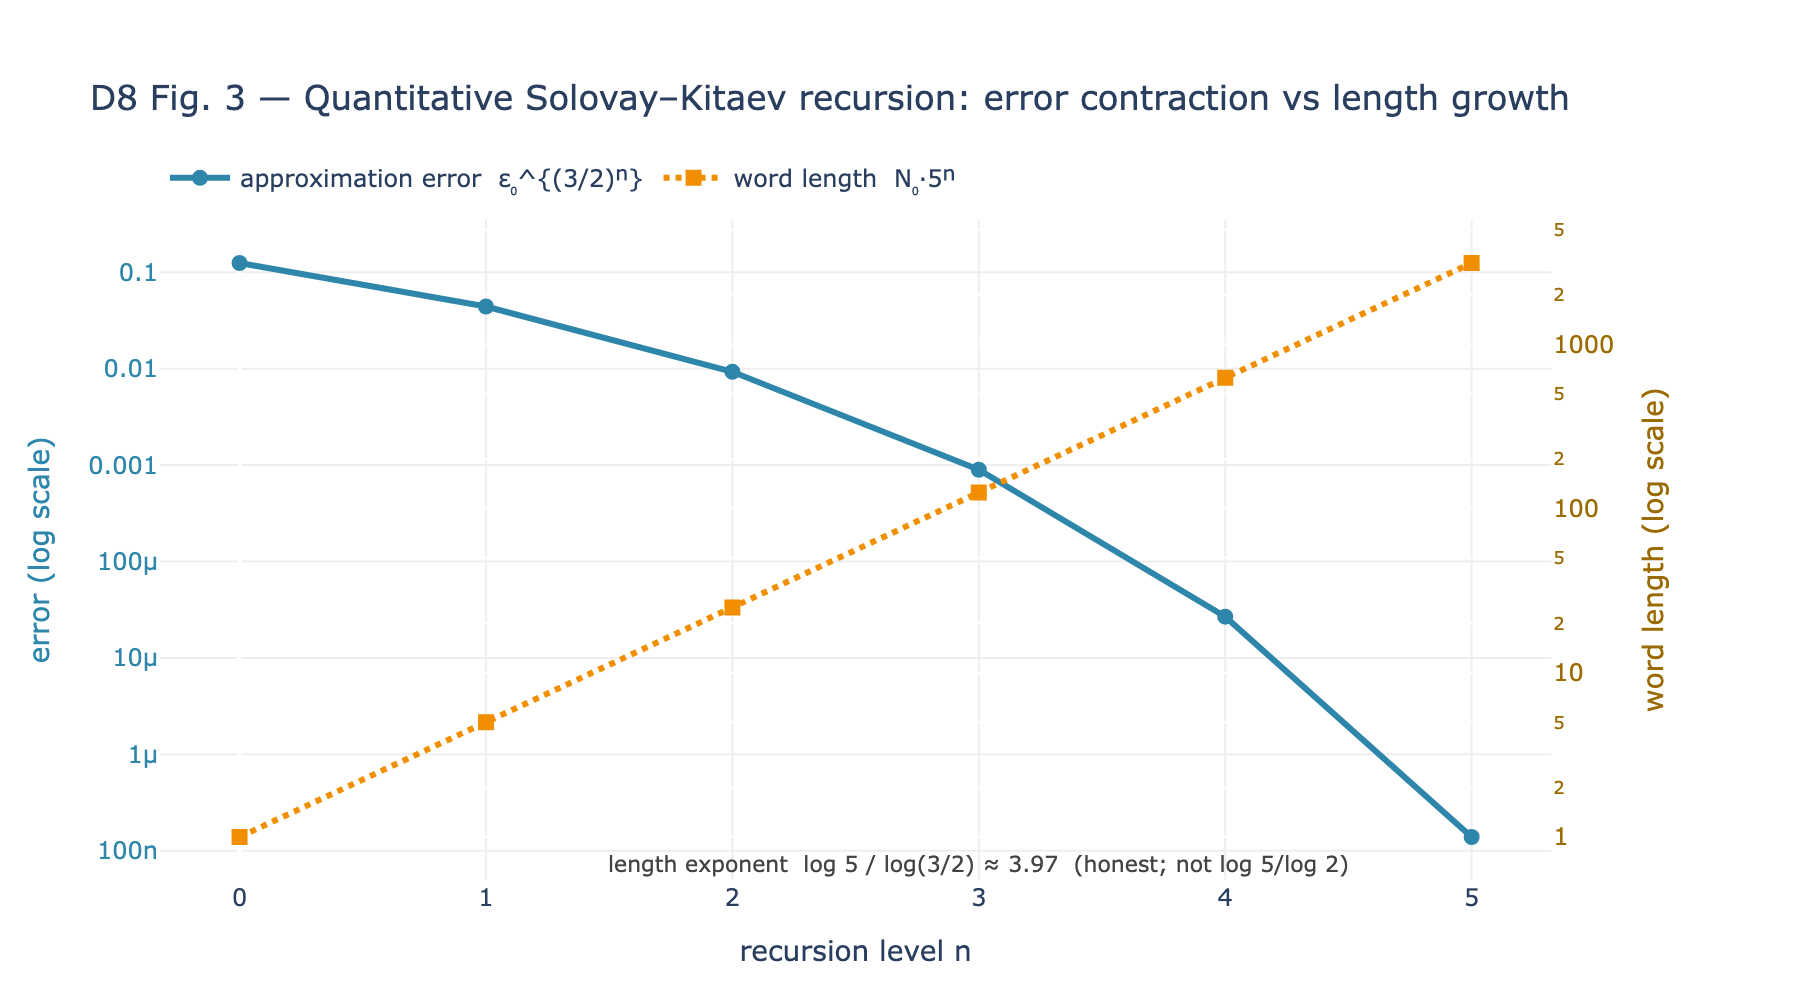
\includegraphics[width=\columnwidth]{figures/d8_fig3_sk_recursion.png}
\caption{The balanced-commutator recursion. Per level the error contracts
super-quadratically as $\varepsilon_0^{(3/2)^n}$ while the word length grows
fivefold from its base value, giving the length exponent
$\gamma = \log 5/\log(3/2) \approx 3.97$~\cite{Selinger2015,KMM2013ancilla}.}
\label{fig:recursion}
\end{figure}

\section{What a new alphabet costs}
\label{sec:alphabets}

The claim of Sec.~\ref{sec:substrate} is that adding a universal alphabet to
the verified chain is an instantiation problem rather than a re-derivation
problem. This section is the evidence. The measure of the claim is not how many
alphabets appear but how much of each one's work is alphabet-specific, so
Table~\ref{tab:alphabets} is organized by that column.

\begin{table}
\caption{What each alphabet supplies. Every entry inherits the recursion, the
net, the Baker--Campbell--Hausdorff estimate and the Cartan step from
Theorem~\ref{thm:substrate} or Theorem~\ref{thm:sud}. The rightmost column is
the whole of the alphabet-specific work.}
\label{tab:alphabets}
\begin{ruledtabular}
\begin{tabular}{lll}
Alphabet & Target & Alphabet-specific input \\
\colrule
Clifford$+T$ & $\su 2$ & $\sqrt 2 \sin(\pi/8)$ not an algebraic integer \\
Read--Rezayi $k=5$ & $\su 2$ & Chebyshev factorization of $T_7(x)+1$ \\
Read--Rezayi $k=7$ & $\su 2$ & triple-angle collapse at $\cos(\pi/9)$ \\
Trapped-ion M\o lmer--S\o rensen & $\su 4$ & Brylinski entangling criterion \\
Clifford$+$CCZ (with $T$) & $\su 8$ & density of the $\{H,T,\mathrm{CNOT}\}$ part \\
Clifford$+$CCZ ($T$-free) & $\su 8$ & $\mathrm{tr} = 1/\sqrt2$ not an algebraic integer \\
\end{tabular}
\end{ruledtabular}
\end{table}

\figuredeferred{fig:d8-coverage}{the existing alphabet-by-dimension coverage
figure shows a Fibonacci row, which Ref.~\cite{RoehmD4Topological} owns and
this paper no longer claims; recutting it against
Table~\ref{tab:alphabets} requires a regenerated figure from the project's
canonical visualization module}

The two Read--Rezayi rows are the sharpest evidence for the interface claim,
because their number theory is genuinely unlike the Clifford$+T$ case and the
interface absorbs it unchanged. We give both.

\paragraph{Read--Rezayi at $k=5$.} The Read--Rezayi states at filling
$\nu = k/(k+2)$ are the non-Abelian fractional quantum Hall family beyond
Fibonacci~\cite{ReadRezayi1999}. At $k = 5$ the relevant braid generator has
trace $2\cos(\pi/7)$, and the obstruction is that $\cos(\pi/7)$ satisfies a
cubic rather than a quadratic. The route is the Chebyshev identity
\[
  T_7(x) + 1 \;=\; (x+1)\,\big(8x^3 - 4x^2 - 4x + 1\big)^2 ,
\]
whose right-hand factor is the minimal polynomial of $2\cos(\pi/7)$ up to
normalization. A finite-order element would force $2\cos(\pi/7)$ into a
cyclotomic field of degree incompatible with that cubic, so the element has
infinite order and the density witness follows.

\paragraph{Read--Rezayi at $k=7$.} At $k = 7$ the corresponding angle is
$\pi/9$, and the obstruction is different in kind: it is not that the minimal
polynomial has large degree but that the triple-angle identity
$\cos(3\cdot \pi/9) = \cos(\pi/3) = 1/2$ pins $\cos(\pi/9)$ as a root of
$4x^3 - 3x = 1/2$, which is irreducible over $\mathbb{Q}$. The same
finite-order contradiction then applies.

Neither argument touches the recursion, the net, the
Baker--Campbell--Hausdorff estimate or the Cartan step. Both produce a
quantitative compilation theorem of the shape of Theorem~\ref{thm:cliffordt},
unconditionally.

\paragraph{Trapped-ion M\o lmer--S\o rensen at $\su 4$.} The two-qubit gate set
realized on production trapped-ion hardware consists of single-qubit rotations
together with the M\o lmer--S\o rensen entangling gate at a discrete grid of
angles. Here the density witness is supplied not by a trace obstruction but by
the Brylinski--Brylinski criterion~\cite{Brylinski2002}: a two-qubit gate $V$,
together with all single-qubit gates, generates a dense subgroup of $\su 4$ if
and only if $V$ is \emph{primitive}, meaning it maps some product state to an
entangled one. The M\o lmer--S\o rensen gate at any angle that is not a
multiple of $\pi$ is entangling by inspection of its action on
$\lvert 00\rangle$, so the criterion applies directly and the alphabet-specific
work reduces to exhibiting one such angle in the grid. The resulting
compilation theorem holds for every even grid resolution $N > 0$ and is
unconditional. This row is the strongest evidence that the interface is not
tuned to number theory: the witness here is geometric, and it enters through
the same predicate as the others.

\paragraph{Clifford$+$CCZ at $\su 8$.} The three-qubit case admits two density
mechanisms that are structurally different, and the contrast between them is
itself a result. Sec.~\ref{sec:su8} treats it separately.

\section{The three-qubit case: CCZ is necessary, sufficient, and priced}
\label{sec:su8}

At $\su 8$ the question stops being whether a compilation exists and becomes
which gate is doing the work. The doubly controlled-$Z$ gate is the expensive
resource in a fault-tolerant architecture, so its role is worth settling
precisely rather than assuming. The channel representation settles all three
parts of the question: that CCZ is necessary, that it is sufficient without
$T$, and what it costs.

\subsection{Sufficient, with \texorpdfstring{$T$}{T}: the over-complete route}

Take the alphabet $\{H, T, \mathrm{CNOT}, \mathrm{CCZ}\}$. Density follows from
the $\{H, T, \mathrm{CNOT}\}$ part alone: single-qubit Clifford$+T$ is dense in
each qubit's $\su 2$ by Theorem~\ref{thm:accpt}, and CNOT couples the factors,
in the manner of the stabilizer analysis of Aaronson and
Gottesman~\cite{AaronsonGottesman2004}. Feeding that witness through
Theorem~\ref{thm:sud} gives an unconditional compilation theorem at $\su 8$.

We flag the scope of that result rather than leaving it to be discovered. In
this route CCZ is present in the alphabet and absent from the proof. The
theorem says the alphabet is universal; it says nothing about CCZ.

\subsection{Sufficient, without \texorpdfstring{$T$}{T}: the CCZ-seeded route}

Now delete $T$. The alphabet is $\{H, S, \mathrm{CNOT}, \mathrm{CCZ}\}$, which
contains no gate outside the Clifford group except CCZ itself.

\begin{theorem}[$T$-free density at $\su 8$]
\label{thm:literal}
The group generated by $\{H, S, \mathrm{CNOT}, \mathrm{CCZ}\}$ is dense in
$\su 8$.
\end{theorem}

The mechanism is not the one above, and the difference is the point. There is
no per-qubit infinite-order element to find, because every single-qubit element
of this alphabet is Clifford and the single-qubit Clifford group is finite. The
argument instead runs globally, in four steps.

First, the seed. Consider $\mathrm{CCZ}\cdot(H\otimes H\otimes H)$. Its
normalized trace is $1/\sqrt 2$, which is not an algebraic integer, so by the
argument of Sec.~\ref{sec:substrate-cliffordt} the seed has infinite order.

Second, from infinite order to a flow. Compactness of $\su 8$ turns the
infinite-order seed into an accumulation point at the identity, and the Cartan
step converts that into a one-parameter subgroup whose generator is a nonzero
element $X$ of the Lie algebra $\mathfrak{su}(8)$.

Third, spreading. Expand $X$ in the Pauli basis. Since $X$ is traceless and
nonzero it has a nonzero coefficient on some non-identity Pauli operator
$P$. The Clifford group acts on the $63$ non-identity Pauli operators of three
qubits by conjugation, and that action is transitive. Conjugating the flow
generated by $X$ by Clifford elements therefore transports the component along
$P$ to every one of the $63$ Pauli directions.

Fourth, closing. The $63$ non-identity Pauli operators span $\mathfrak{su}(8)$.
A closed connected subgroup of a compact connected Lie group whose Lie algebra
is the whole algebra is the whole group, so the closure of the generated
subgroup is $\su 8$, which is Definition~\ref{def:dense}. Feeding
Theorem~\ref{thm:literal} through Theorem~\ref{thm:sud} gives an unconditional
$T$-free compilation theorem at $\su 8$.

\subsection{Necessary: the Clifford group alone is finite}

Theorem~\ref{thm:literal} shows CCZ suffices. It does not by itself show CCZ is
doing anything, since a redundant generator can be added to an already dense
set. The converse supplies the missing half.

\begin{theorem}[Clifford-only is not dense]
\label{thm:notdense}
The group generated by $\{H, S, \mathrm{CNOT}\}$ is not dense in $\su 8$.
\end{theorem}

The proof is the channel representation. Write $\widehat U$ for the matrix of
the map $P \mapsto U P U^{\dagger}$ in the Pauli basis. On the Clifford group
this map sends Pauli operators to Pauli operators up to sign, so $\widehat U$
is a signed permutation matrix. Signed permutation matrices of fixed size form
a finite group, so the image of the Clifford group under the channel
representation is finite, and a subgroup with finite image cannot be dense in
$\su 8$.

Taken together, Theorems~\ref{thm:literal} and~\ref{thm:notdense} settle the
role of CCZ at $\su 8$: it is not over-complete, and the two density routes of
this section are not two proofs of one fact but proofs about two different
alphabets, one of which is universal only because CCZ is in it.

\begin{figure*}
\centering
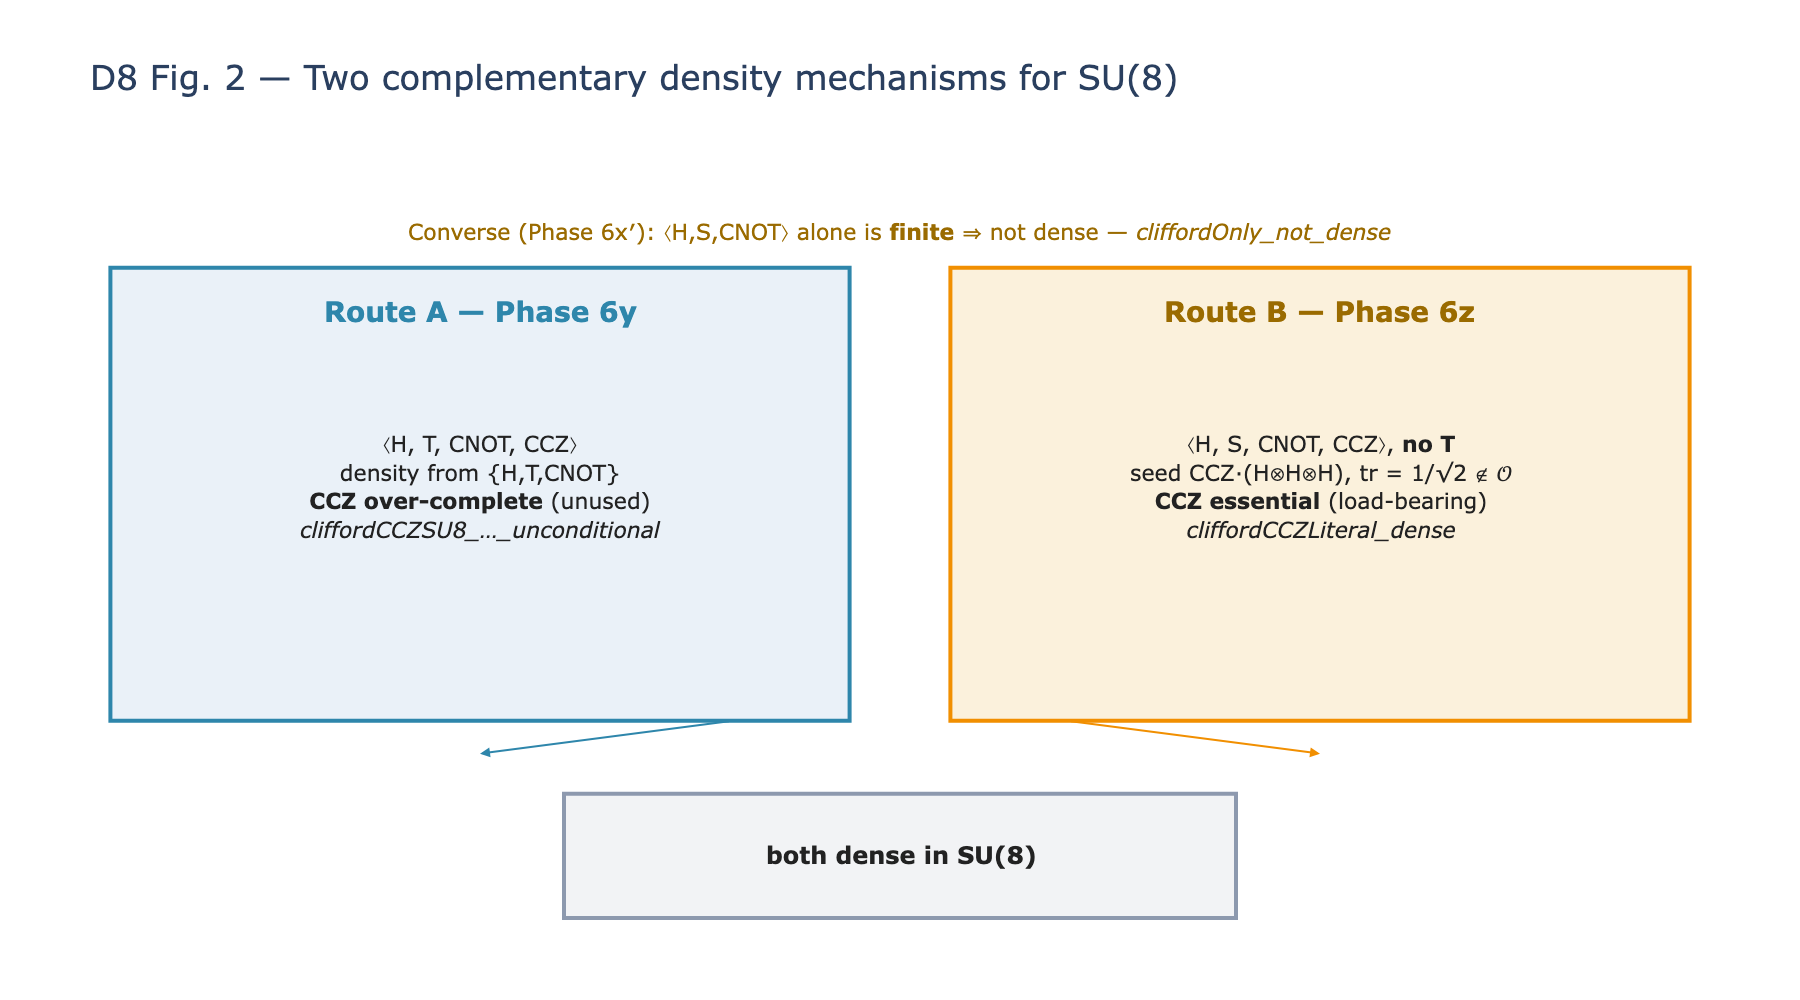
\includegraphics[width=0.86\textwidth]{figures/d8_fig2_su8_density_duality.png}
\caption{Two formally verified density mechanisms for the same target $\su 8$.
The upper route is $T$-based, with CCZ present in the alphabet and absent from
the proof. The lower route is $T$-free, with density seeded by
$\mathrm{CCZ}\cdot(H\otimes H\otimes H)$ and spread by Clifford conjugation
across the $63$ non-identity Pauli operators. The converse
(Theorem~\ref{thm:notdense}) establishes that the Clifford group alone has
finite image under the channel representation, so CCZ is the resource that
makes the difference.}
\label{fig:su8duality}
\end{figure*}

\subsection{Priced: a verified Toffoli-count lower bound}
\label{sec:resource}

The same representation that proves Theorem~\ref{thm:notdense} also prices CCZ.
For a rational number $q$ let
\[
  \mathrm{sde}_2(q) \;=\; \max\big(0,\, -v_2(q)\big),
\]
where $v_2$ is the $2$-adic valuation, so that $\mathrm{sde}_2(q)$ is the
exponent of $2$ in the denominator of $q$ in lowest terms, and $0$ when the
denominator is odd. Extend it to a matrix with rational entries by taking the
maximum over entries, and write $\mathrm{sde}_2(\widehat U)$ for its value on
the channel representation. Write $T^{\mathrm{of}}(U)$ for the least number of
CCZ (equivalently Toffoli) gates in any exact Clifford$+$CCZ circuit for $U$,
defined as an infimum over all such circuits.

\begin{theorem}[Toffoli-count lower bound]
\label{thm:toffoli}
Let $U$ be exactly implementable by some Clifford$+$CCZ circuit. Then
$\mathrm{sde}_2(\widehat U) \le T^{\mathrm{of}}(U)$.
\end{theorem}

The proof telescopes three facts, following the resource theory of
Mukhopadhyay~\cite{Mukhopadhyay2024}: $\mathrm{sde}_2(\widehat{\mathbf 1}) = 0$;
$\mathrm{sde}_2$ does not increase under multiplication by a Clifford gate,
because the channel representation of a Clifford is a signed permutation and
permuting entries does not change the maximum; and $\mathrm{sde}_2$ increases
by at most one under a CCZ, because CCZ's channel-representation rows are
half-integral. Any circuit with $m$ CCZ gates therefore reaches
$\mathrm{sde}_2$ at most $m$ from a start of $0$, and taking the infimum over
circuits gives the theorem.

For $\mathrm{sde}_2$ to be defined at all the entries must be rational, and
that is a theorem: the channel-representation entries of any Clifford$+$CCZ
word are rational. It is worth being precise about what is and is not needed
here, because Mukhopadhyay's corresponding lemma states the stronger dyadic
conclusion that the entries lie in $\mathbb Z[1/2]$. The $2$-adic valuation is
defined on all of $\mathbb Q$, so $\mathrm{sde}_2$, its behaviour under
Clifford multiplication, and its increment under CCZ are all established at the
level of rationals, and Theorem~\ref{thm:toffoli} needs nothing more. What the
dyadic refinement buys is interpretive rather than logical: it is what makes
$\mathrm{sde}_2(\widehat U)$ readable as a smallest-denominator exponent in a
dyadic ring rather than merely as the $2$-part of a rational denominator. The
lower bound holds either way.

Two scope statements. The bound is stated for unitaries exactly implementable
in Clifford$+$CCZ, which is the domain on which $T^{\mathrm{of}}$ is meaningful.
And the matching upper bound, that is minimality, is not addressed: establishing
it requires the meet-in-the-middle search behind Mukhopadhyay's Conjecture~4.8,
and the lower bound stands on its own without it.
% TODO: Mukhopadhyay2024 (arXiv:2401.08950) is held as a project-authored
% abstract summary, not as source text. The section, lemma and conjecture
% numbers cited here follow the formalization's internal cross-references and
% have not been checked against the paper itself. Acquire the primary source
% before this bundle goes green.

\section{From existence to an algorithm}
\label{sec:compiler}

Everything above certifies that a good compilation \emph{exists}. That is
weaker than what a compiler user wants, in a specific and checkable way: an
existence statement is compatible with there being no procedure that finds the
word. This section closes the gap for Clifford$+T$, which is the alphabet where
closing it matters most.

The object is a single named function
\[
  \mathrm{cliffordTCompile} \colon \su 2 \times \mathbb R \longrightarrow
    \mathrm{FreeGroup}(\mathrm{Fin}\,2),
\]
taking a target and a precision to a word in the free group on the two
generators $H$ and $T$. Its verification has the shape of a loop-correctness
proof, and each part is a separate statement.

\begin{lemma}[Termination at finite depth]
\label{lem:compile-term}
For every $U$ and $\varepsilon$, $\mathrm{cliffordTCompile}(U,\varepsilon)$
equals the structural balanced-commutator recursion run to depth
$n(\varepsilon) = \lceil \log_{3/2}\big(\log_4 (1/(K^2\varepsilon))\big)\rceil$.
\end{lemma}

Because the recursion is structural in the depth, termination is by
construction rather than by a measure argument. Lemma~\ref{lem:compile-term} is
what makes the remaining statements about a function rather than about a
process.

\begin{lemma}[Initialization]
\label{lem:compile-base}
At depth $0$ the compiler returns the word produced by the constructive base
finder.
\end{lemma}

\begin{lemma}[Loop invariant]
\label{lem:compile-inv}
At every depth $n$ and for every target $U$, the depth-$n$ output approximates
$U$ within the super-quadratically shrinking budget
$\varepsilon_n = K^{-2}\,(K^2\varepsilon_0)^{(3/2)^n}$. The invariant holds
unconditionally, for all $n$ and all $U$ simultaneously.
\end{lemma}

\begin{theorem}[Compiler correctness]
\label{thm:compile}
For every $U \in \su 2$ and every $\varepsilon \in (0,\varepsilon_0]$, the word
$W = \mathrm{cliffordTCompile}(U,\varepsilon)$ satisfies all three of:
\begin{enumerate}
\item $\opn{\rho(W) - U} \le \varepsilon$;
\item $L\big(n(\varepsilon)\big) \le c\,(\log 1/\varepsilon)^{\gamma}$, where
$L$ is the recursion-level length function;
\item $\lvert W\rvert \le \Lambda\big(m, n(\varepsilon)\big)$, where $\lvert
W\rvert$ is the reduced word length of the emitted word, $m$ is the maximum
word length in the constructive $\varepsilon_0$-cover, and $\Lambda$ is an
explicit closed form in $m$ and the depth.
\end{enumerate}
\end{theorem}

Conjuncts (ii) and (iii) are different objects and the distinction is
load-bearing. Conjunct (ii) bounds a length \emph{recurrence}, the quantity
$L(n+1) = 5L(n) + \mathrm{const}$ that the analysis of
Sec.~\ref{sec:sud-exponent} solves; it is the statement that the recursion is
poly-logarithmic. Conjunct (iii) bounds the length of the word the function
actually returns. A reader who takes the substrate's poly-logarithmic conjunct
to be a bound on emitted output is reading conjunct (ii) as conjunct (iii), and
only Theorem~\ref{thm:compile} supplies the latter.

Two limitations, stated rather than left to be found. The constant in (iii) is
the constructive $\varepsilon_0$-cover's maximum word length, not the
information-theoretically optimal constant, which is precisely the gap
Sec.~\ref{sec:length} addresses. And the accompanying worked instantiation,
which witnesses that the contract is not vacuous, is evaluated at $U = \mathbf 1$
and $\varepsilon = \varepsilon_0$, that is at the identity target and the base
precision, so it exercises the contract at recursion depth $0$ and not beyond.

Finally, the scope boundary. The compiler is a mathematical function inside the
proof assistant, verified once for all inputs. Engineering it into a runnable,
performance-tuned piece of software is a separate deliverable and is not
attempted here.

\section{How long is the circuit: three mechanisms, three honesties}
\label{sec:length}

The recursion of Sec.~\ref{sec:sud-exponent} delivers word length
$O\big((\log 1/\varepsilon)^{3.97}\big)$. The information-theoretic optimum is
$O(\log 1/\varepsilon)$, exponent $1$, and closing that gap is what separates a
theoretically adequate compiler from a usable one. Three mechanisms are
verified here, and no one of them dominates the others. Each buys the exponent
at a different price, and the three prices are the honest content of this
section.

\begin{table}
\caption{The three verified compilation mechanisms. No mechanism is best on
every axis; the table is the comparison a compiler author actually needs.}
\label{tab:mechanisms}
\begin{ruledtabular}
\begin{tabular}{llll}
Mechanism & Exponent & Conditional on & Ancillas \\
\colrule
Balanced commutator & $3.97$ & nothing & none \\
Ross--Selinger grid & $1$ & Hypothesis~\ref{hyp:residual} & none \\
Kliuchnikov--Maslov--Mosca & $1$ & nothing & two \\
\end{tabular}
\end{ruledtabular}
\end{table}

\figuredeferred{fig:d8-length-comparison}{a figure comparing the three verified
length bounds as functions of precision, plotted directly from the theorem
statements of this section, requires a plotting function in the project's
canonical visualization module; the bounds themselves are proved and appear in
Table~\ref{tab:mechanisms}}

\subsection{The grid route and its one hypothesis}
\label{sec:length-rs}

For $z$-rotations, Ross and Selinger~\cite{RossSelinger2016} achieve the
optimal exponent by reducing approximate synthesis to a lattice problem over
the ring $\mathbb Z[\omega]$, $\omega = e^{i\pi/4}$, and then solving an exact
synthesis problem over $\mathbb Z[\omega][1/\sqrt 2]$ in the manner of
Kliuchnikov, Maslov and Mosca~\cite{KMM2013}. We verify the efficiency layer of
that route.

\begin{theorem}[Grid-route length]
\label{thm:rslength}
Suppose the grid finder succeeds at precision parameter $k$ and bound $b$,
returning $t$. Then the synthesized Clifford$+T$ word satisfies
\[
  \lvert W\rvert \;\le\; N_3 + 16\log_2(1/\delta) + 16\log_2(1+\sqrt 2),
  \qquad \delta = \frac{1+\sqrt 2}{\sqrt 2^{\,k}},
\]
equivalently $\lvert W\rvert \le N_3 + 8k$, where $N_3$ is the fixed word-length
overhead of the exact-synthesis step. This is $O(\log 1/\varepsilon)$ with
exponent $1$.
\end{theorem}

The conditionality is not left as an atmosphere. It reduces to a single
statement, which we state as a hypothesis so that it can be inspected.

\begin{hypothesis}[Bounded residual realization]
\label{hyp:residual}
For a grid candidate $u$ and precision parameter $k$ there exists
$t \in \mathbb Z[\omega]$ of bounded height with
$t^{\dagger}t = 2^k - u^{\dagger}u$.
\end{hypothesis}

\begin{theorem}[The hypothesis suffices]
\label{thm:rssynth}
Hypothesis~\ref{hyp:residual} implies that the grid finder succeeds, and
delivers the full conclusion of Theorem~\ref{thm:rslength} with
$\lvert W\rvert \le N_3 + 8k$.
\end{theorem}

Theorem~\ref{thm:rssynth} isolates the gap exactly. What is known about
Hypothesis~\ref{hyp:residual} is this. The source
literature discharges it as a randomized algorithm under a prime-distribution
assumption, which appears as Hypothesis~8.3 of Ref.~\cite{RossSelinger2016} and,
in the same form, as Hypothesis~29 of Ref.~\cite{Selinger2015}. An
unconditional discharge would require the existence of relative norms of
prescribed form in growing windows, which is a short-interval statement in
analytic number theory. Hypothesis~\ref{hyp:residual} is strictly weaker than
the prime-distribution assumption, since it asks for a relative norm rather
than a prime. It is open in the formalized-mathematics ecosystem, and in its
primality form it is open in the literature.

Hypothesis~\ref{hyp:residual} appears in the statement of every theorem that
consumes it. It is never an axiom, so the zero-project-local-axiom property of
this development is unaffected, and Theorems~\ref{thm:rslength}
and~\ref{thm:rssynth} are kernel-checked exactly as stated.

\subsection{The Diophantine substrate underneath}
\label{sec:length-appc}

Theorem~\ref{thm:rssynth} rests on the solvability theory for
$t^{\dagger}t = \xi$ over $\mathbb Z[\omega]$, which we verify as a chain
rather than assuming. The chain is worth exhibiting because it is where the
number theory actually lives.

Here $\dagger$ is the ring automorphism of $\mathbb Z[\omega]$ sending
$\omega \mapsto \omega^{-1}$, an element $\xi$ of the fixed ring
$\mathbb Z[\sqrt 2]$ is \emph{doubly positive} when it is positive under both
real embeddings $\sqrt 2 \mapsto \pm\sqrt 2$, and $\xi$ is
\emph{$\dagger$-decomposable} when it is a relative norm $t^{\dagger}t$ for some
$t \in \mathbb Z[\omega]$. Solvability is thus decomposability, and the chain
below reduces decomposability to a congruence condition on prime factors.

\begin{lemma}[Units]
\label{lem:c2}
A unit of $\mathbb Z[\sqrt 2]$ that is positive under both real embeddings is a
square.
\end{lemma}

Lemma~\ref{lem:c2} is what makes the criterion below independent of the choice
of associate: the unit group of $\mathbb Z[\sqrt 2]$ is generated by $-1$ and
the fundamental unit $1+\sqrt 2$, whose norm is $-1$, so a doubly positive unit
has even exponent on the fundamental unit and is therefore a square. Without
it, decomposability could fail merely because a representative was multiplied by
a unit.

\begin{lemma}[Solvability criterion]
\label{lem:c16}
$t^{\dagger}t = \xi$ is solvable in $\mathbb Z[\omega]$ if and only if $\xi$ is
doubly positive and $\dagger$-decomposable.
\end{lemma}

Double positivity is necessary because a relative norm is a sum of squares under
each real embedding. That it is, with decomposability, also sufficient is the
content, and it is a biconditional rather than an implication, which is what
lets the grid search reject a candidate rather than merely fail to accept it.

\begin{lemma}[Multiplicativity]
\label{lem:c19}
$\dagger$-decomposability is multiplicative across coprime factors: a product of
coprime factors is $\dagger$-decomposable if and only if each factor is.
\end{lemma}

Lemma~\ref{lem:c19} is what turns the criterion into a decision procedure: it
reduces a question about $\xi$ to independent questions about the prime powers
in its factorization. The two lemmas that follow answer those questions.

\begin{lemma}[The obstruction at $p \equiv 7 \bmod 8$]
\label{lem:c20}
An element whose norm is a power of a prime $p \equiv 7 \pmod 8$ is not
$\dagger$-decomposable when that power is odd, and for a prime dividing the
norm squared there is a constructive decomposition in the remaining cases.
\end{lemma}

The congruence class is not arbitrary: $2$ ramifies in $\mathbb Z[\sqrt 2]$ and
the splitting of an odd prime $p$ is governed by whether $2$ is a quadratic
residue modulo $p$, which holds exactly for $p \equiv \pm 1 \pmod 8$. The
residue class $7 \bmod 8$ is the one where $p$ splits in $\mathbb Z[\sqrt 2]$
but the resulting primes fail to be relative norms from $\mathbb Z[\omega]$, and
a mod-$8$ count of the valuation is what detects it.

\begin{lemma}[Even-power criterion]
\label{lem:c21}
For $\xi$ of norm $\pm p$ with $p \equiv 7 \pmod 8$, the power $\xi^m$ is
$\dagger$-decomposable if and only if $m$ is even.
\end{lemma}

Lemma~\ref{lem:c21} is again a biconditional, and it closes the chain: combined
with Lemma~\ref{lem:c19} it decides decomposability for any $\xi$ whose
factorization is known, which is what the grid finder needs at each candidate.

The greatest-common-divisor machinery these lemmas consume requires that
$\mathbb Z[\omega] = \mathbb Z[\zeta_8]$ be a Euclidean domain, an instance
absent from Mathlib and supplied here. The structure must be taken on
$\mathbb Z[\omega]$ itself and not on the subring $\mathbb Z[\sqrt 2][i]$,
which is an index-$2$, non-integrally-closed subring and therefore not even a
unique factorization domain.

On the geometric side, the one-dimensional grid-existence input is sharpened to
the form the two-disk analysis actually consumes.

\begin{lemma}[Grid existence, product form]
\label{lem:grid}
If $\delta\Delta \ge (1+\sqrt 2)^2$ then a grid point exists at every position,
where the naive centre-rounding argument requires \emph{both} interval lengths
to be at least $1+\sqrt 2$ separately.
\end{lemma}

Lemma~\ref{lem:grid} is what makes the asymmetric case usable, in which a tiny
$\varepsilon$-region is paired against a large disk and neither interval alone
meets the naive bound while their product does.

% TODO: RossSelinger2016 (arXiv:1403.2975) is not held by this project in any
% form; the Appendix-C lemma numbering, the Hypothesis 8.3 reference and the
% Lemma 4.4 attribution above are taken from the formalization's internal
% cross-references and from secondary deep-research notes, not from the paper.
% The mathematical statements are the formalization's own and are kernel-checked;
% the attributions are not verified. Acquire the primary source before green.

\subsection{The ancilla route, unconditionally}
\label{sec:length-kmm}

The wall of Sec.~\ref{sec:length-rs} is number-theoretic, and it can be walked
around rather than climbed. Kliuchnikov, Maslov and
Mosca~\cite{KMM2013ancilla} observed that adjoining ancilla qubits changes the
Diophantine problem the synthesis must solve: instead of a two-square condition
over $\mathbb Z[\omega]$, one obtains a four-square problem, and Lagrange's
theorem solves four-square problems always. No prime density is needed anywhere.

\begin{theorem}[Ancilla-assisted synthesis]
\label{thm:kmm}
For every $U \in \su 2$ and every $k \in \mathbb N$ there exist a three-qubit
Clifford$+T$ word $W$ with
\[
  \lvert W\rvert \;\le\; 50400\,k + 812
\]
and a phase $c$ with $\lvert c\rvert = 1$, such that for every unit pair
$(\alpha,\beta)$, applying $W$ to
$(\alpha\lvert 0\rangle + \beta\lvert 1\rangle)\otimes\lvert 00\rangle$
produces a state within squared $\ell^2$ distance
\[
  9\left(\frac{2}{4^k} + \frac{2\sqrt 2}{2^k}\right)
\]
of $(c^{-1}U(\alpha\lvert 0\rangle + \beta\lvert 1\rangle))\otimes\lvert 00\rangle$.
\end{theorem}

The error scale is $\varepsilon \sim 2^{-k}$ up to constants, so the length is
$O(\log 1/\varepsilon)$ with exponent exactly $1$, unconditionally. The proof
combines Lagrange's four-square theorem with a constructive dimension-four
column lemma in the style of the exact-synthesis analysis of Giles and
Selinger~\cite{GilesSelinger2013}, and a verified Euler $Z$--$X$--$Z$
decomposition of $\su 2$.

Three properties of Theorem~\ref{thm:kmm} distinguish it from
Theorems~\ref{thm:substrate} and~\ref{thm:rslength}, and all three matter
downstream. It is a \emph{state-level} contract: the guarantee is on the image
of ancilla-initialized input states, with the ancillas restored in the
comparison state, and it is not a bound on the operator-norm distance between
$W$'s unitary and $U$. It carries a global phase $c$, which is physically
irrelevant but is present in the statement. And the constants $50400$ and $812$
are verified upper bounds on the construction implemented here, not optimized
ones and not constants extracted from Ref.~\cite{KMM2013ancilla}, whose own
statement is asymptotic. Tightening them is engineering.

The first of these three properties has a consequence that
Sec.~\ref{sec:diamond} must confront: an operator-norm bound is what converts
into a channel-level guarantee, so of the three mechanisms only the recursion
route currently reaches the physical layer.

\section{From compiled word to physical channel}
\label{sec:diamond}

Every bound so far constrains the distance between two matrices. What a
hardware error budget consumes is the distance between two \emph{channels}, in
the worst case over all inputs including entangled ones. The gap between the
two is not a formality, and closing it is what makes a synthesis bound usable
as a certificate.

For a unitary $U$ let $\Phi_U(\rho) = U\rho U^{\dagger}$, and let
$\mathrm{diamondDist}$ denote the supremum, over density operators $\rho$ on
the system tensored with an ancilla of equal dimension, of the trace distance
between the stabilized outputs. This is the $\tfrac12\lVert\cdot\rVert_\diamond$
convention.

\begin{theorem}[Operator norm to diamond distance]
\label{thm:akn}
For unitaries $U$ and $V$,
$\mathrm{diamondDist}(\Phi_U, \Phi_V) \le \opn{U - V}_{2}$,
where $\opn{\cdot}_2$ is the $\ell^2$ operator norm. Equivalently
$\lVert \Phi_U - \Phi_V\rVert_\diamond \le 2\opn{U-V}_2$.
\end{theorem}

Theorem~\ref{thm:akn} is the conversion of Aharonov, Kitaev and
Nisan~\cite{AKN1998}. The proof telescopes an add-and-subtract identity and is
established for arbitrary contractions, which is strictly more general than the
unitary case needs. Two supporting bounds carry the dimensional bookkeeping: the
ancilla register is handled by the Kronecker bound
$\opn{A \otimes \mathbf 1}_2 \le \opn{A}_2$, and the trace-norm H\"older
inequalities are transferred from the community quantum-information
library~\cite{Meiburg2025PhysLib} through a single identification of that
library's trace norm with the one used here.

A known limitation is shipped as a theorem rather than as a remark: the bound
is not tight under global phase. Specifically,
$\mathrm{diamondDist}(\Phi_{e^{i\theta}U}, \Phi_U) = 0$ for every $\theta$,
while $\opn{e^{i\theta}U - U}_2$ is positive. Phase-optimized tightening is
therefore available and is not claimed here.

\begin{theorem}[End-to-end channel certificate]
\label{thm:capstone}
For every $U \in \su 2$ and every $\varepsilon \in (0,\varepsilon_0]$, writing
$W = \mathrm{cliffordTCompile}(U,\varepsilon)$,
\[
  \mathrm{diamondDist}\big(\Phi_{\rho(W)},\, \Phi_U\big) \;\le\;
    \sqrt 2\,\varepsilon .
\]
\end{theorem}

Each link is checked. Theorem~\ref{thm:compile}(i) gives an $\ell^\infty$
operator-norm bound, that is a bound of $\varepsilon$ on every row sum. A
row-sum-to-$\ell^2$ bridge converts this to
$\opn{\rho(W) - U}_2 \le \sqrt{\mathrm{card}}\;\varepsilon = \sqrt 2\,\varepsilon$
at one qubit, and Theorem~\ref{thm:akn} finishes. The $\sqrt 2$ is the
dimensional constant of the norm bridge and not the conversion constant; a
sharper bridge would improve it.

The scope of Theorem~\ref{thm:capstone} should be read against
Table~\ref{tab:mechanisms}. It composes with the compiler of
Sec.~\ref{sec:compiler}, whose contract is an operator-norm bound. The grid
route of Sec.~\ref{sec:length-rs} produces exact-synthesis words and would
compose similarly once its hypothesis is discharged, but the ancilla route of
Sec.~\ref{sec:length-kmm} carries a state-level contract, and lifting a
state-level guarantee to a diamond-distance guarantee is not done here. Of the
three verified length mechanisms, one currently reaches the channel layer.

\section{The trust boundary}
\label{sec:trust}

A verification paper owes its reader an account of what was checked, by what,
and what remains outside. This section is that account.

\subsection{What the kernel checked}

Every theorem stated in this paper is verified to the Lean~4 kernel with axiom
set $\{\texttt{propext},\allowbreak \texttt{Classical.choice},\allowbreak
\texttt{Quot.sound}\}$, which is the standard Lean kernel, and with no
project-local axioms. Conditional statements, meaning Theorems~\ref{thm:sud},
\ref{thm:rslength} and~\ref{thm:rssynth}, carry their hypotheses in the theorem
statement and are kernel-checked exactly as stated.

Lean offers two ways to discharge a large finite check. The tactic
\lean{decide} evaluates inside the kernel. The tactic \lean{native\_decide}
compiles the check and runs it, which extends the trusted base from the kernel
to the Lean compiler and the host toolchain. The exact-synthesis layer beneath
Sec.~\ref{sec:length-kmm} originally rested on four \lean{native\_decide}
sweeps, the largest of them over roughly $16.7$ million tuples. All four have
been replaced by structural arguments, and one of the replacements is a result
in its own right.

\begin{lemma}[Orthogonality kills a column]
\label{lem:somekills}
For an orthogonal triple in the relevant $\mathbb Z[\omega]$ lattice, some
column-reduction step strictly decreases the height.
\end{lemma}

Lemma~\ref{lem:somekills} replaces an exhaustive sweep over orthogonal triples
with a parity argument in the style of Giles and
Selinger~\cite{GilesSelinger2013}, and in doing so it \emph{strengthens} the
statement: the hypothesis the sweep required is not needed by the parity
argument and has been dropped. The other three replacements are a
parity-and-ramification calculus for the bridge step, a torsion classification
of small-norm $\mathbb Z[\omega]$ elements that reduces the Clifford base case
to chunked kernel-checked \lean{decide}s, and a pairing-form calculus that
reduces the mod-$8$ valuation algebra to two kernel-checked sweeps. The corpus
this paper reports contains no compiled-evaluation escape.

\subsection{What the Lean statements do and do not say}

Four places where a natural reading of a theorem's name is stronger than the
theorem, collected here rather than left distributed.

The substrate's poly-logarithmic conjunct at $\su 2$ is a bound on the
recursion-level length function, and the bound on the emitted word is
Theorem~\ref{thm:compile}(iii). The Toffoli lower bound
(Theorem~\ref{thm:toffoli}) holds for unitaries exactly implementable in
Clifford$+$CCZ, which is where its right-hand side is defined. The
ancilla-assisted synthesis (Theorem~\ref{thm:kmm}) is a state-level contract on
ancilla-initialized inputs, not an operator-norm statement. And the worked
instantiation accompanying Theorem~\ref{thm:compile} is evaluated at the
identity target and the base precision, so it witnesses non-vacuity at
recursion depth $0$.

\subsection{What is outside}

Three sources this paper cites are not held by the project in full text, and
the affected attributions are marked in the manuscript source. They are the
grid-synthesis paper of Ross and Selinger, the exact-synthesis paper of
Kliuchnikov, Maslov and Mosca, and the resource-theory paper of Mukhopadhyay.
In each case the mathematical statements formalized here are the formalization's
own and are kernel-checked; what is unverified is the correspondence between
those statements and the section, lemma and hypothesis numbers under which the
sources state them.

\section{Scope and outlook}
\label{sec:scope}

What this paper establishes is the verified existence, universality,
algorithm-correctness, optimal-length synthesis, and lower-bound theory of
universal quantum gate compilation: that a compilation exists with provable
error and length bounds at arbitrary dimension for the alphabets treated here;
that a named compilation algorithm meets its contract as a theorem
(Sec.~\ref{sec:compiler}); that exponent-$1$ synthesis is verified along two
further mechanisms with their conditionality made precise
(Sec.~\ref{sec:length}); that a compiled gate carries a channel-level
certificate (Sec.~\ref{sec:diamond}); and that the CCZ resource is necessary,
sufficient and priced at $\su 8$ (Sec.~\ref{sec:su8}).

What is not in scope is the engineering of a runnable compiler: the runtime
implementation, hardware-specific tuning, certificate formats, and
constant-factor optimization, including tightening the verified $50400k + 812$
bound of Sec.~\ref{sec:length-kmm} toward practical $T$-counts. Two
mathematical boundaries are also open and are stated where they arise:
Hypothesis~\ref{hyp:residual}, on which ancilla-free exponent-$1$ synthesis
rests; and the lifting of a state-level synthesis contract to a diamond-distance
guarantee, without which the ancilla route does not reach the channel layer.

The methodological claim is the one worth carrying forward. By separating what
is alphabet-specific from what is not, and lifting the latter to arbitrary
dimension, the cost of verifying a new universal gate set reduces to a single
density witness, and Sec.~\ref{sec:alphabets} shows that witnesses as different
as an algebraic-integer obstruction, a Chebyshev factorization, a triple-angle
identity and an entangling-gate criterion all pass through the same interface
unchanged. The $\su 8$ result suggests a further use: formal verification here
is not only checking known compilation results but settling a structural
question, namely whether a gate is doing work in a universality proof, that is
easy to state and delicate to answer.

\paragraph{Companion work.} The Fibonacci braid representation, its density in
$\su 2$, and the topological and categorical foundations of anyonic computation
are developed in Ref.~\cite{RoehmD4Topological}, which owns the Fibonacci
alphabet and is the origin point of the algebraic-integer technique reused
throughout Sec.~\ref{sec:alphabets}. The channel and measurement certification
layer that Sec.~\ref{sec:diamond} consumes, including the operator-norm bounds
supporting Theorem~\ref{thm:akn}, is developed in
Ref.~\cite{RoehmD9Certification}. The fault-tolerant code and logic substrate
that consumes the compilation primitive proved here is developed in
Ref.~\cite{RoehmD6FaultTolerant}.

\appendix

\section{Verification status}
\label{app:verification}

Every theorem in this paper is verified to the Lean~4 kernel with axiom set
$\{\texttt{propext}, \texttt{Classical.choice}, \texttt{Quot.sound}\}$ and no
project-local axioms. No statement is discharged by an axiom or by compiled
evaluation; every finite check in the corpus is kernel-checked
(Sec.~\ref{sec:trust}).

Theorem~\ref{thm:substrate} is \lean{GenericSU2} and \lean{GenericSUd}
\lean{SolovayKitaevHeadline}; Theorem~\ref{thm:accpt} is
\lean{cliffordT\_accPt\_one\_unconditional}; Theorem~\ref{thm:cliffordt} is
\lean{solovayKitaev\_dawson\_nielsen\_quantitative\_cliffordT\_strict\_constructive\_tight\_unconditional};
Theorem~\ref{thm:mercator} is \lean{exp\_matrixMercatorLog};
Theorem~\ref{thm:sud} is
\lean{solovayKitaev\_dawson\_nielsen\_quantitative\_generic\_sud\_strict\_constructive\_tight};
Theorem~\ref{thm:literal} is \lean{cliffordCCZLiteral\_dense};
Theorem~\ref{thm:notdense} is \lean{cliffordOnly\_not\_dense};
Theorem~\ref{thm:toffoli} is \lean{channelSde2\_le\_toffoliCost}, with entry
rationality \lean{channelRep\_interp\_isRat}; Theorem~\ref{thm:compile} is
\lean{cliffordTCompile\_correct}, with Lemmas~\ref{lem:compile-term},
\ref{lem:compile-base} and~\ref{lem:compile-inv} being
\lean{cliffordTCompile\_eq\_recursion},
\lean{cliffordTCompile\_recursion\_base} and
\lean{cliffordTCompile\_loop\_invariant};
Theorem~\ref{thm:rslength} is \lean{rossSelinger\_log\_length\_explicit};
Hypothesis~\ref{hyp:residual} enters through
\lean{gridFindT\_isSome\_of\_residual} and Theorem~\ref{thm:rssynth} is
\lean{rossSelinger\_synth\_of\_residual}; Lemmas~\ref{lem:c2}--\ref{lem:c21} are
\lean{zsqrt2\_isSquare\_of\_unit\_pos\_pos},
\lean{relNorm\_iff\_doublyPositive\_decomposable},
\lean{daggerDecomposable\_mul\_iff},
\lean{not\_daggerDecomposable\_of\_norm\_pow\_seven},
\lean{daggerDecomposable\_of\_prime\_dvd\_normSq} and
\lean{daggerDecomposable\_pow\_iff\_seven};
Lemma~\ref{lem:grid} is \lean{oneDim\_grid\_exists\_product};
Theorem~\ref{thm:kmm} is \lean{kmm\_universal\_headline};
Theorem~\ref{thm:akn} is \lean{diamondDist\_unitaryKraus\_le};
Theorem~\ref{thm:capstone} is \lean{diamondDist\_cliffordTCompile\_le}; and
Lemma~\ref{lem:somekills} is \lean{someKills\_of\_orthogonal}.

\section{Reusable components}
\label{app:reusable}

Several components of this development are general-purpose and are absent from
Mathlib at the pin used here.

\begin{table}[h]
\caption{Components with use beyond this development.}
\label{tab:reusable}
\begin{ruledtabular}
\begin{tabular}{ll}
Component & Where it arises \\
\colrule
Banach-algebra logarithm, named radius & Theorem~\ref{thm:mercator} \\
Euclidean domain instance for $\mathbb Z[\zeta_8]$ & Sec.~\ref{sec:length-appc} \\
Euler $Z$--$X$--$Z$ decomposition of $\su 2$ & Sec.~\ref{sec:length-kmm} \\
Dimension-generic BCH order-two cubic estimate & Sec.~\ref{sec:substrate} \\
$\su d$ Cartan density-from-witness lemma & Sec.~\ref{sec:sud} \\
Matrix-exponential local homeomorphism at $\mathbf 1$ & Sec.~\ref{sec:sud} \\
\end{tabular}
\end{ruledtabular}
\end{table}

The elimination of compiled evaluation described in Sec.~\ref{sec:trust} is a
precondition for any of these being contributed upstream, since
\lean{native\_decide} is not accepted there.

\bibliography{bibliography}
\bibliographystyle{apsrev4-2}

\end{document}
